\section{Synteza dźwięku fletu}

W literaturze można znaleźć wiele podejść do syntezy dźwięku instrumentów dętych drewnianych. Ich modele są przedstawione zazwyczaj za pomocą różniczkowych równań fizycznych lub w postaci falowodów cyfrowych. 
%klarnet: https://www.researchgate.net/publication/4333455_Representation_of_solo_clarinet_music_by_physical_modeling_synthesis
%gestures: https://www.researchgate.net/publication/5323798_Gesture_synthesis_basic_control_of_a_flute_physical_model
%slide-flute perry cook: https://quod.lib.umich.edu/cache//b/b/p/bbp2372.1992.072/bbp2372.1992.072.pdf#page=1;zoom=75
Przykładem takiej pracy naukowej jest artykuł na temat modelu fizycznego klarnetu, w którym autorzy opisują równaniami różniczkowymi poszczególne elementy instrumentu dętego drewnianego \cite{flute_klarnet}. Inna praca naukowa porusza temat kontroli modelu fletu, w którym autorzy skupili się na opisaniu zależnościach fizycznych związanych z grą flecisty \cite{flute_flecista}, takich jak: ciśnienie w ustach instumentalisty, odległość od fletu oraz szerokość otwarcia ust. Kolejnym przykładem artykułu opisującego model instrumentu dętego drewnianego jest praca P. Cooka przedstawiająca falowody cyfrowe fletu suwakowego (ang. slide flute) oraz klarnetu \cite{flute_cook}.

%o tym ze trudno jest zrobić wielootworowe --> ta ksiazka computer music costam


W niniejszym podrozdziale przedstawiono dwa podejścia do implementacji syntezy dźwięku drewnianego instrumentu dętego:
\begin{itemize}
	\setlength\itemsep{-3pt}
	\item za pomocą falowodu cyfrowego,
	\item za pomocą zidentyfikowanego modelu ARMA.
\end{itemize}
Na końcu podrozdziału przedstawiono porównanie wyników obu tych podejść do syntezy, na podstawie wygenerowanych dźwięków.

\subsection{Synteza falowodowa}
%https://ccrma.stanford.edu/~jos/pasp/Digital_Waveguide_Models.html
%https://quod.lib.umich.edu/cache//b/b/p/bbp2372.1992.072/bbp2372.1992.072.pdf#page=1;zoom=75

Synteza falowodowa instrumentów dętych drewnianych opiera się głównie na cyfrowych liniach opóźniających, które symulują odbicia fali w komorze dźwiękowej (ang. bore) tego rodzaju instrumentów. Komorę dźwiękową można uprościć do cylindra, w którym rozchodzi się fala. Jest to znaczna zaleta metody falowodowej, gdyż dowolny element instrumentu może zostać zamodelowany za pomocą zestawu tub cylindrycznych.

\begin{equation} \label{equ:flute_row_falowe}
\frac{\partial^2 p}{\partial t^2} = \frac{\partial^2 p}{\partial x^2}
\end{equation}
\begin{tabular}{ l l l l}
	gdzie: 	&	$p$ & - &  ciśnienie, \\
	& $c$ &  - & prędkość propagacji dźwięku w powietrzu, \\
	&	$x$ & - &  długość korpusu instrumentu dętego,\\
	&	$t$ & - &  czas, \\
\end{tabular} \\

%https://sound.eti.pg.gda.pl/student/eim/synteza/macmal/
Jednowymiarowe równanie falowe (\ref{equ:flute_row_falowe}) przedstawia rozchodzenie się fali płaskiej w nieskończenie długim cylindrze. Rozwiązaniem równania jest superpozycja dwóch fal ciśnienia (fal dźwiękowych) rozchodzących się w przeciwnych kierunkach komory dźwiękowej instrumentu dętego.


\subsubsection{Model}
W niniejszej pracy, syntezę falowodową dźwięku instrumentu dętego drewnianego oparto o schemat blokowy przedstawiony przez P. Cooka w 1992 roku.

\begin{figure}[H]
	\centering
	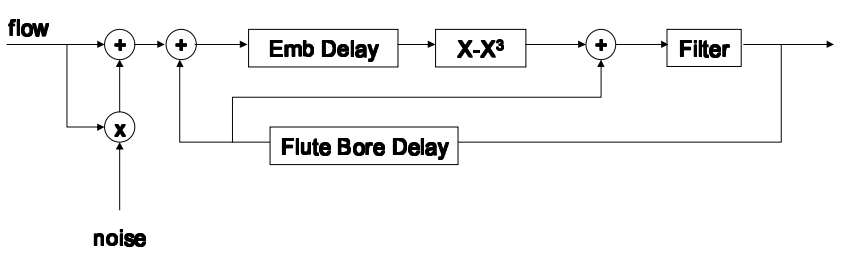
\includegraphics[width=14cm]{grafiki/flute_waveguide_mod}
	\captionsetup{justification=centering}
	\caption{Model falowodowy prostego instrumentu dętego drewnianego.}
	\label{rys:flute_cook}
\end{figure}

%https://courses.cs.washington.edu/courses/cse467/05wi/pdfs/lectures/15-waveguideInstruments.pdf
Wejściem systemu przedstawionego na rysunku \ref{rys:flute_cook} jest przepływ powietrza. Szum zostaje dodany w celu symulowania odgłosu wydechu flecisty. 
Interakcja między ustnikiem a komorą dźwiękową fletu przedstawiona została równaniem matematycznym $x-x^3$. Końcówka komory dźwiękowej fletu odbija niskie częstotliwości - ta część została zasymulowana poprzez dodanie filtru dolnoprzepustowego przed wyjściem sygnału. Elementy "Emb Delay" oraz "Flute Bore Delay" to linie opóźniające, odpowiadające opóźnieniom fali w ustniku oraz komorze dźwiękowej. 
Obliczenie jednej próbki syntezowanego dźwieku na podstawie rysunku \ref{rys:flute_cook} wymaga 9 mnożeń oraz 6 operacji sumowania.

\subsubsection{Implementacja}
Implementację syntezy falowodowej w autorskim programie realizowanym na procesorze DSP,  wzorowano również na schemacie \ref{rys:flute_cook}. Przepływ powietrza został zaimplementowany jako jedna fala sinusoidalna o odpowiedniej obwiedni \cite{flute_prezka}. Szum dochodzący do utworzonego sygnału został zasymulowany funkcją rand(), a jego ilość została zeskalowana. Sygnały sinusoidy i szumu są sumowane, a następnie trafiają do pętli zamkniętej, którą zaimplementowano w postaci pętli "for".

Jeden blok danych na procesorze DSP zawiera 1024 próbek. Linie opóźniające przesuwają próbki o kilkadziesiąt indeksów. Oznacza to, iż pierwsza próbka nowego bloku danych, musi sięgnąć do poprzednio wygenerowanej tablicy. Taki mechanizm został zaimplementowany jako dwie tablice. Po wygenerowaniu pełnego bloku danych, pierwsza tablica przepisuje wszystkie wartości do drugiej. Następnie pierwsza tablica zostaje wyzerowana. Wszystkie opóźnione próbki, do których należy się odnieść przy generowaniu nowego bloku danych, znajdują się w drugiej tablicy. Takim mechanizmem zapewniono ciągłość generowania sygnału w zależności od próbek z przeszłości.

\subsection{Synteza na podstawie modelu ARMA}
W tym punkcie przedstawiono identyfikację modelu matematycznego fletu, na podstawie którego przeprowadzono później syntezę dźwięku. Do rozpoznania modelu instrumentu użyto tonu "A" razkreślnego o częstotliwości 440Hz. Dźwięk wygenerowany przez grę na flecie zmienia swoją charakterystykę w czasie. Oznacza to, iż jego model również zmienia się w trakcie nagranego przebiegu sygnału. Do identyfikacji wybrano te część nagrania dźwięku fletu, w której model instrumentu jest w stanie ustalonym.

\subsubsection{Identyfikacja modelu}
Identyfikacja modelu matematycznego instrumentu została przeprowadzona poprzez manualne dopasowanie zer i biegunów modelu.
Proces identyfikacji przeprowadzono w środowisku symulacyjnym Matlab. Na nagranym fragmencie sygnału przeprowadzono dyskretną transformację Fouriera za pomocą algorytmu FFT.

Identyfikacja procesu modelem wysokiego rzędu za pomocą funkcji wbudowanych w środowisku Matlab dawała lepsze rezultaty niż manualne szukanie pików i dolin. Taki sposób nie pozwalał jednak na późniejszą parametryzację modelu dla różnych dźwięków. Z tego powodu, autorzy zrezygnowali w automatycznej identyfikacji modelu ARMA.

% WYKRESSSSS
\begin{figure}[H]
	\centering
	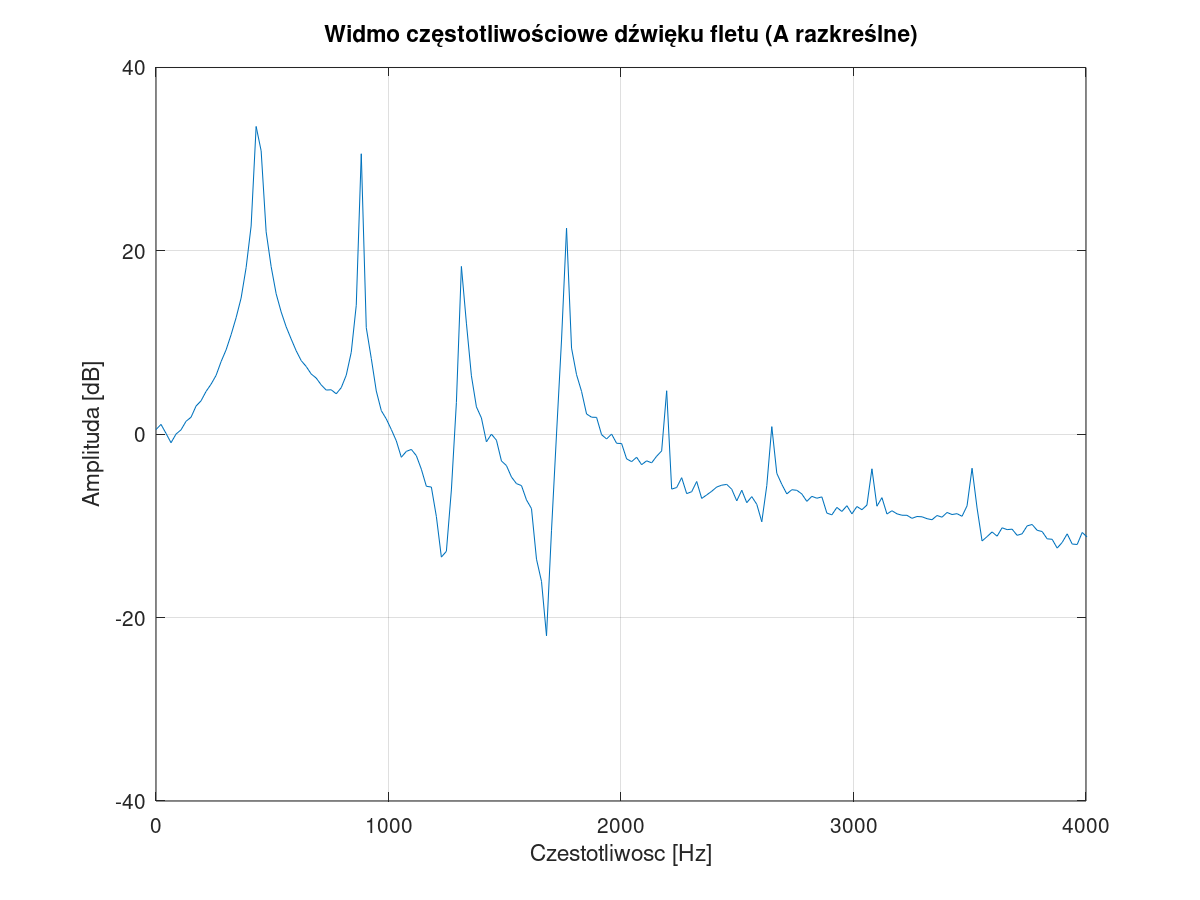
\includegraphics[width=12cm]{grafiki/flute_spectrum_orig}
	\captionsetup{justification=centering}
	\caption{Charakterystyka amplitudowa nagranego sygnału fletu.}
	\label{rys:flute_spectrum}
\end{figure}
% WYKRESSSS

Na rysunku \ref{rys:flute_spectrum} można zauważyć wyraźne piki oraz doliny charakterystyki częstotliwościowej nagranego sygnału. Siedem pierwszych pików charakterystyki zostało zinterpretowanych jako bieguny modelu, natomiast sześć pierwszych dolin zostały potraktowane jako jego zera. Liczba wybranych pików i dolin wziętych pod uwagę przy tworzeniu modelu, została dobrana na podstawie wzrokowej oceny ilości harmonicznych mogących mieć znaczny wpływ na ukształtowanie brzmienia zsyntezowanego instrumentu. Częstotliwości rezonansowe przetworzono według zależności:
\begin{equation} \label{equ:flute_bieguny}
p = 1-\frac{0.05}{A_{p}}e^{jf_{p}2\pi/F_{s}}
\end{equation}
\begin{equation} \label{equ:flute_doliny}
q = 1-\frac{0.05}{A_{q}}e^{jf_{q}2\pi/F_{s}}
\end{equation}
\begin{tabular}{ l l l l}
	gdzie: & $p$ &  - & bieguny modelu, \\
	&	$q$ & - &  zera modelu, \\
	&	$F_{s}$ & - &  częstotliwość próbkowania nagranego dźwięku,\\
	&	$f_{p,q}$ & - &  częstotliwość rezonansowa biegunów i zer modelu, \\
	&	$A_{p,q}$ & - &  amplituda rezonansu zer i biegunów, \\
\end{tabular} \\

Każdy pik charakterystyki został przetworzony na dwa bieguny odbite lustrzanie względem osi rzeczywistej na płaszczyźnie Z, według wzoru (\ref{equ:flute_bieguny}). Każda z dolin została odwzorowana jako dwa zera odbite lustrzanie względem osi Z, według wzoru (\ref{equ:flute_doliny}).

Model ARMA zsyntezowanego fletu utworzono na podstawie wyznaczonych zer i biegunów. W celu wygenerowania dźwięku z modelu w środowisku symulacyjnym, pobudzono go szumem białym. Następnie znormalizowano otrzymany sygnał, aby uniknąć przesterowań. Dźwięk wygenerowany z modelu przypominał brzmienie instrumentu z rodziny instrumentów dętych drewnianych. Wysokość wygenerowanego dźwięku jest taka sama jak w oryginalnym nagraniu (440Hz).

\subsubsection{Parametryzacja zidentyfikowanego modelu}
Gra na instrumencie wymaga wydobywania z niego dźwięków o różnej wysokości. Zidentyfikowany w poprzednim punkcie model jest statyczny - po pobudzeniu modelu szumem, wydobywa się z niego zawsze dźwięk o tej samej częstotliwości podstawowej ("A" razkreślny, na podstawie którego, model był identyfikowany). W celu wydobycia innego tonu na podstawie utworzonego modelu, należy dokonać jego parametryzacji. Parametryzacja zidentyfikowanego modelu polega na uzależnieniu każdego biegunu i zera modelu od pożądanego tonu.

Parametryzacja modelu opierać się będzie o zasady przyjęte w protokole MIDI. 
Na podstawie wzoru (\ref{equ:wpr_dzwiek}), każdy biegun został uzależniony od częstotliwości podstawowej zidentyfikowanego modelu. Częstotliwość podstawowa wymnożona przez pierwiastek dwunastego stopnia podniesiony do potęgi różnicy półtonów między częstotliwością 440Hz a częstotliwością pożądanego dźwięku pozwoliła utworzyć bieguny oraz zera w odpowiednim miejscu.
\begin{figure}[H]
	\centering
	\includegraphics[width=12cm]{grafiki/Model_B_A}
	\label{rys:por_mod_flet}
	\captionsetup{justification=centering}
	\caption{Porównanie widma modeli ARMA fletu dla dzwieku "B" razkreślnego (wykres przesuniety w prawo) i "A" razkreślnego (wykres przesunięty w lewo).}
	\label{rys:por_mod_flet}
\end{figure}
Na rysunku \ref{rys:por_mod_flet} widać, iż wszystkie piki oraz doliny opisane zidentyfikowanym modelem przesuwają się w dziedzinie częstotliwości dla różnych tonów. Oznacza to, iż pobudzony model wyda dźwięk o różnej wysokości dla różnych parametrów wejściowych.


\subsubsection{Implementacja}
W autorskim programie na procesorze DSP, syntezę dźwięku za pomocą zidentyfikowanego modelu ARMA, zaimplementowano jako przetwarzanie szumu przez filtr IIR. Współczynniki filtru pobrano z przeprowadzonej wcześniej symulacji w środowisku Matlab. Sygnałem wyjściowym był generowany dźwięk instrumentu dętego.

% opisac jak zaimplementowano filtr IIR ??
% O tym jak precyzja zmieniala wyniki!! Na floatach nie dziala.

Algorytm wystawiania kolejnych bloków danych z próbkami dźwięku jest taki sam, jak opisany w podrozdziale || REF IMPLEMENTACJA KUBY W FM ||.

Interfejs użytkownika metody fizycznej ogranicza się jedynie do włączenia syntezy fletu na procesorze DSP. Nie ma możliwości zmian parametrów modeli przez użytkownika.

\subsection{Wyniki}
Poniżej przedstawiono wyniki syntezy fletu dla obu metod - falowodowej oraz poprzez model ARMA.

\begin{figure}[H]
	\centering
	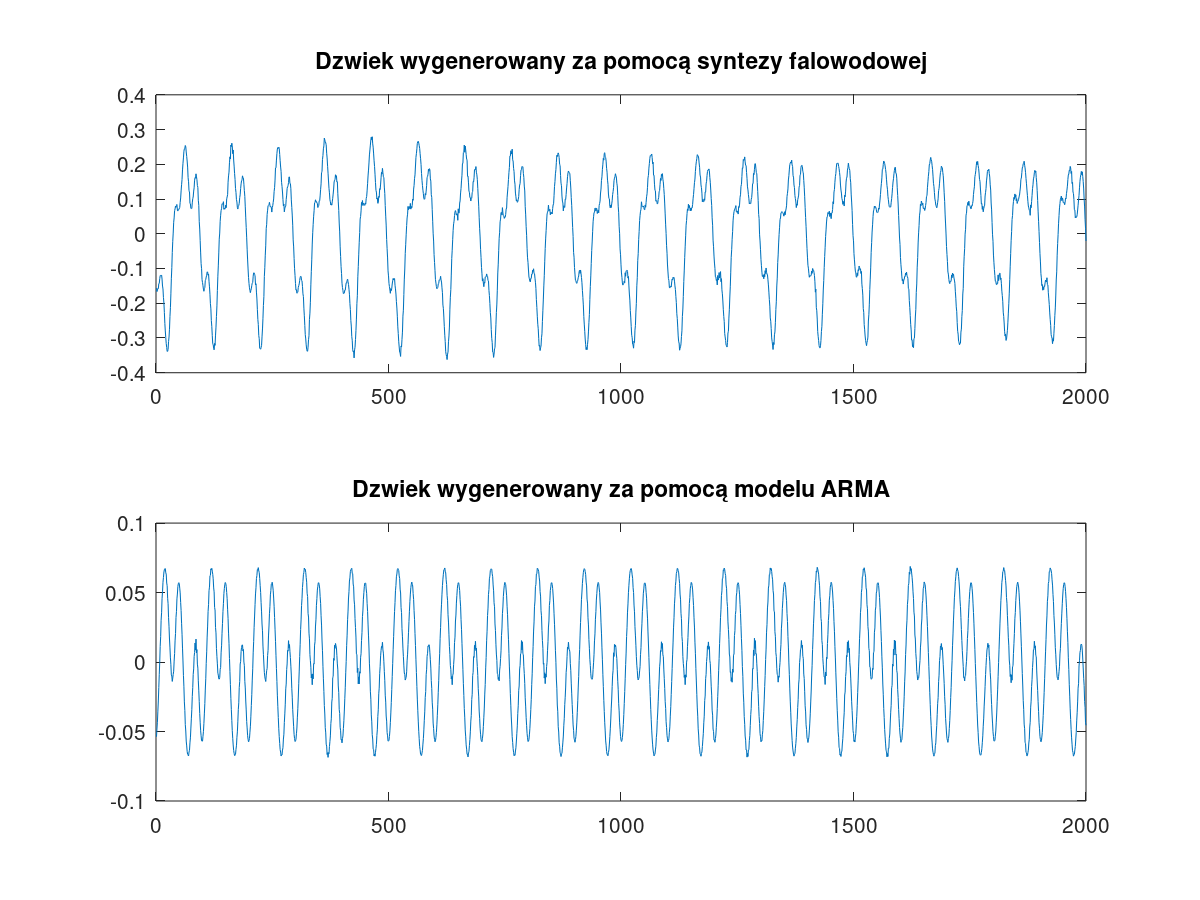
\includegraphics[width=12cm]{grafiki/flute_porownanie_syntez_symulacja}
	\captionsetup{justification=centering}
	\caption{Porównanie symulacji dzwieku fletu dla syntezy falowodowej i syntezy za pomocą modelu ARMA fletu.}
	\label{rys:por_synt_flet}
\end{figure}

Można zauważyć, iż porównanie syntezy instrumentu dętego, które zostało przedstawione na rysunku \ref{rys:por_synt_flet}, dało zupełnie różne wyniki dla obu metod. Po odpowiednim doborze parametrów, brzmienie uzyskane metodą syntezy falowodowej jest bliższe barwy fletu. W celu otrzymania lepszych wyników syntezą za pomocą modelu ARMA, należałoby prawdopodobnie użyć modelu zmiennego w czasie.
